\documentclass[12pt]{article}

\usepackage{hyperref}
\usepackage{graphicx}
\graphicspath{{./img/}}

\pagenumbering{arabic}

% VARIABLES
\def\UART_VERSION{v1.0.0}

\begin{document}
\begin{titlepage}
  \centering
  {\LARGE \textsc{Uart Implementation Reference}\par}
  {\vspace{1cm}}
  \UART_VERSION \\
  {\vspace{16cm}}
  Written by \\
  Kevin LASTRA
\end{titlepage}
\tableofcontents
\newpage

\section{Introduction}

\subsection{Purpose of the manual}
The purpose of this manual is twofold. First, it serves as a 
comprehensive resource to document the Implementation of a 
Universal Asynchronous Receiver-Transmitter (UART). This process 
has been undertaken not only as a journey of self-learning but also 
as a way to share knowledge and contribute to the broader community
of developers, engineers, and enthusiasts.

\subsection{Audience}
This manual is primarly intended for design engineers who are 
involved in the development and implementation of communication
systems, particularly those working with embedded systems, 
microcontrollers, and hardware interfaces.

\newpage
\section{UART overview}
The Universal Asynchronous Receiver-Transmitter (UART) is a 
fundamental hardware communication protocol used for asynchronous
serial communication. \\
This protocol is widely used in embedded systems, 
microcontrollers, and communication devices due to its simplicity and effectiveness
in handling relatively low-speed data transfer.
\subsection{UART fundamentals}
\subsubsection{Reception and transmission}
UART allows two devices to exchange data using only two wires, RX for receive data
and TX for transmit data.\\
\begin{figure}[h]
  \centering
  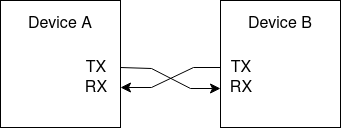
\includegraphics[scale=0.6]{UART_interface.drawio.png}
  \caption{Two UART's interfaces connected}
\end{figure}


\subsubsection{Asynchronous communication}
An asynchronous communication refers to a type of data transmission where the sender
and receiver do not rely on a shared clock signal for synchronization. Instead, each
device operates using its own internal clock and relies on specific timing 
conventions to ensure data is transmitted and received correctly. \\~\\
In asynchronous UART communication, the data is sent in discrete chunks 
(called data frames) over the communication channel, with the timing governed by 
agreed-upon parameters like baud rate and frame size.

\subsubsection{Baud rate}
The baud rate defines the speed at which data is transmitted over the communication
channel. It is usually expressed in bits per second (bps). \\
In the context of UART the baud rate specifies how many bits of data can be 
transmitted each second. Both transmitter and receiver must be set to the same baud
rate. \\~\\
The general formula for calculating the baud rate is:

\[Baud Rate = \frac{Clock Frequency}{Divisor}\]

\subsubsection{Data frame structure}
A UART data frame typically consists of: \\

\begin{table}[h]
  \centering
  \begin{tabular}{|p{3cm}|p{6cm}|p{3.5cm}|}
    \hline
    \textbf{Range name} & \textbf{Description} & \textbf{Implementation bit length} \\
    \hline
    Start bit & Signals the beginning of data transmission & 1 \\
    \hline
    Data bits & The actual data being sent & 5 - 9 \\
    \hline
    Parity & Used for error checking & 0 - 1 \\
    \hline
    Stop bit & Signals the end of the data transmission & 1 - 2 \\
    \hline
  \end{tabular}
\end{table}

\subsection{Advantages and limitations}
Advantages:
\begin{enumerate}
  \item Minimal pins required, essay to implement on a system.
  \item Low cost, because of its minimal hardware requirements the UART is a
        cost-effective solution.
  \item Widely supported.
  \item Simplicity in software implementation.
\end{enumerate}
limitations:
\begin{enumerate}
  \item Distance limitations, the maximum range depends on the baud rate, the quality
        of the wires and the environment (e.g. electromagnetic interferences).
  \item Relatively slow data transfer.
  \item Limited to two devices.
  \item Susceptibility to baud rate mismatch.
  \item Limited error detection, UART error detection is limited to parity checks and
        stop bits.
\end{enumerate}

\section{Implementation}
\begin{figure}[h]
  \centering
  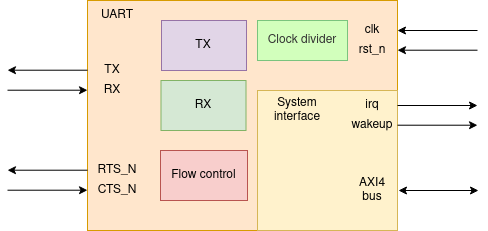
\includegraphics[scale=0.6]{UART_IMPL_DIAGRAM.drawio.png}
  \caption{Implementation diagram}
\end{figure}
\subsection{Design}
\subsection{Interface}
\subsubsection{UART}
The UART interface includes the basic two wires for data transmission and reception
\textbf{rx} and \textbf{tx}.\\
In addition to the basic lines, the UART interface includes two control flow lines:
\begin{enumerate}
  \item RTS\_N \textbf{(Ready to Send)}: Signals that the device is ready to send data.
  \item CTS\_N \textbf{(Clear to Send)}: Indicate that the receiving device is ready 
        to accept data.
\end{enumerate}
\textbf{Why use cts\_n and rts\_n?}\\~\\
The flow control solve two principal issues:
\begin{enumerate}
  \item Overflow, a fast transmitter could overwhelm a slower receiver, leading to 
        data loss or corruption
  \item Collision, when two devices attempt to transmit data simultaneously, it can 
        result in garbled communication or corrupted data.
\end{enumerate}
Without proper flow control, these issues can severely impact communication reliability.
The control flow wires solve this by coordinating the readiness of both devices:
\begin{enumerate}
  \item The transmitter checks \textbf{cts\_n} to ensure the receiver is ready before sending 
        data.
  \item The receiver asserts \textbf{rts\_n} when it is ready to receive more data, allowing 
        the transmitter to proceed.
\end{enumerate}
This approach is especially useful in systems with devices of varying processing
speeds or in applications where reliability is critical, such as industrial 
communication systems or high-throughput embedded designs.
\subsubsection{System}
On the system side, the UART interface is connected to the system using the following
components:\\~\\
\textbf{AXI4 bus}\\~\\
The UART control and configuration are managed through an AXI4 bus interface, a 
widely used protocol in system-on-chip (SoC) designs. The AXI4 bus allows the system
to:\\
\begin{enumerate}
  \item Configure UART parameters.
  \item Monitor UART status registers for errors, activity, or flow control states.
  \item Enable or disable interrupts for data transmission and reception.
\end{enumerate}

\textbf{IRQ lines for RX and TX}\\~\\
To optimize system efficiency, the UART module includes two dedicated interrupt
wires.\\~\\
\textbf{Wakeup line}\\~\\
The wake-up line is used to bring the system out of a low-power or sleep mode when 
activity is detected on the UART interface.
\subsection{Registers}
\subsection{Interrupt request (IRQ)}
\subsection{Low power}

\section{Versioning}
This manual follows a structured versioning system to ensure
clarity and traceability of updates. The version number is 
formatted as vX.Y.Z, where:
\begin{enumerate}
  \item \textbf{X} - major revisions, such as significant updates to 
            content or structure.
  \item \textbf{Y} - minor revisions, such as additions or updates 
            to specific sections.
  \item \textbf{Z} - minor edits, such as corrections to typos, 
            formatting, or small clarifications.
\end{enumerate}
\subsection{History}
\begin{tabular}{|p{1.5cm}|p{1.5cm}|p{2.5cm}|p{7cm}|}
  \hline
  Version & Date & Author & Description \\
  \hline
  v1.0.0 & 0 & Kevin Lastra & Initial release of the UART Implemenation Reference \\
  \hline
\end{tabular}
\section{Glosary}
\section{References}
\end{document}